%%%%%%%%%%%%%%%%%%%%%%%%%%%%%%%%%%%%%%%%%
% Masters/Doctoral Thesis
% LaTeX Template
% Version 2.5 (27/8/17)
%
% This template was downloaded from:
% http://www.LaTeXTemplates.com
%
% Version 2.x major modifications by:
% Vel (vel@latextemplates.com)
%
% This template is based on a template by:
% Steve Gunn (http://users.ecs.soton.ac.uk/srg/softwaretools/document/templates/)
% Sunil Patel (http://www.sunilpatel.co.uk/thesis-template/)
%
% Template license:
% CC BY-NC-SA 3.0 (http://creativecommons.org/licenses/by-nc-sa/3.0/)
%
%%%%%%%%%%%%%%%%%%%%%%%%%%%%%%%%%%%%%%%%%

%----------------------------------------------------------------------------------------
%	PACKAGES AND OTHER DOCUMENT CONFIGURATIONS
%----------------------------------------------------------------------------------------

\documentclass[
12pt, % The default document font size, options: 10pt, 11pt, 12pt
oneside, % Two side (alternating margins) for binding by default, uncomment to switch to one side
english, % ngerman for German
onehalfspacing, % Single line spacing, alternatives: onehalfspacing or doublespacing
%draft, % Uncomment to enable draft mode (no pictures, no links, overfull hboxes indicated)
%nolistspacing, % If the document is onehalfspacing or doublespacing, uncomment this to set spacing in lists to single
%liststotoc, % Uncomment to add the list of figures/tables/etc to the table of contents
%toctotoc, % Uncomment to add the main table of contents to the table of contents
%parskip, % Uncomment to add space between paragraphs
%nohyperref, % Uncomment to not load the hyperref package
headsepline, % Uncomment to get a line under the header
%chapterinoneline, % Uncomment to place the chapter title next to the number on one line
%consistentlayout, % Uncomment to change the layout of the declaration, abstract and acknowledgements pages to match the default layout
]{MastersDoctoralThesis} % The class file specifying the document structure

\usepackage[utf8]{inputenc} % Required for inputting international characters
\usepackage[T1]{fontenc} % Output font encoding for international characters
\usepackage{todonotes}
\usepackage{mathpazo} % Use the Palatino font by default

%\usepackage[style=numeric]{biblatex} % Use the bibtex backend with the authoryear citation style (which resembles APA)
\usepackage[backend=bibtex,style=numeric]{biblatex}
\bibliography{thesis, literature_review/literature_review, project_plan/project_plan}
\nocite{*}

\usepackage[autostyle=true]{csquotes} % Required to generate language-dependent quotes in the bibliography
\usepackage{multirow}
\usepackage{colortbl}

%----------------------------------------------------------------------------------------
%	MARGIN SETTINGS
%----------------------------------------------------------------------------------------

\geometry{
	paper=a4paper, % Change to letterpaper for US letter
	inner=2.5cm, % Inner margin
	outer=3.8cm, % Outer margin
	bindingoffset=.5cm, % Binding offset
	top=1.5cm, % Top margin
	bottom=1.5cm, % Bottom margin
	%showframe, % Uncomment to show how the type block is set on the page
}

%----------------------------------------------------------------------------------------
%	THESIS INFORMATION
%----------------------------------------------------------------------------------------

% Your thesis title, this is used in the title and abstract, print it elsewhere with \ttitle
\thesistitle{Music from Biosignals}
% Your supervisor's name, this is used in the title page, print it elsewhere with \supname
\supervisor{Associate Professor Kenneth \textsc{Pope}}
% Your examiner's name, this is not currently used anywhere in the template, print it elsewhere with \examname
\examiner{}
% Your degree name, this is used in the title page and abstract, print it elsewhere with \degreename
\degree{Bachelour of Engineering (Electronics)(Honours)}
% Your name, this is used in the title page and abstract, print it elsewhere with \authorname
\author{Cooper Wolfden}
% Your address, this is not currently used anywhere in the template, print it elsewhere with \addressname
\addresses{}

% Your subject area, this is not currently used anywhere in the template, print it elsewhere with \subjectname
\subject{Electronic Engineering}
% Keywords for your thesis, this is not currently used anywhere in the template, print it elsewhere with \keywordnames
\keywords{Biosensors}
% Your university's name and URL, this is used in the title page and abstract, print it elsewhere with \univname
\university{\href{https://www.flinders.edu.au/}{Flinders University}}
% Your department's name and URL, this is used in the title page and abstract, print it elsewhere with \deptname
\department{\href{https://www.flinders.edu.au/college-science-engineering}{College of Science and Engineering}}
% Your research group's name and URL, this is used in the title page, print it elsewhere with \groupname
\group{The Douglas Adams Institute For Implausible Linguistics}
% Your faculty's name and URL, this is used in the title page and abstract, print it elsewhere with \facname
\faculty{\href{}{}}

\AtBeginDocument{
\hypersetup{pdftitle=\ttitle} % Set the PDF's title to your title
\hypersetup{pdfauthor=\authorname} % Set the PDF's author to your name
\hypersetup{pdfkeywords=\keywordnames} % Set the PDF's keywords to your keywords
}

\begin{document}

\frontmatter % Use roman page numbering style (i, ii, iii, iv...) for the pre-content pages

\pagestyle{plain} % Default to the plain heading style until the thesis style is called for the body content

%----------------------------------------------------------------------------------------
%	TITLE PAGE
%----------------------------------------------------------------------------------------

\begin{titlepage}
\begin{center}

\vspace*{.06\textheight}
{\scshape\LARGE \univname\par}\vspace{1.5cm} % University name
\textsc{\Large Honours Thesis}\\[0.5cm] % Thesis type

\HRule \\[0.4cm] % Horizontal line
{\huge \bfseries \ttitle\par}\vspace{0.4cm} % Thesis title
\HRule \\[1.5cm] % Horizontal line

\begin{minipage}[t]{0.4\textwidth}
\begin{flushleft} \large
\emph{Author:}\\
{\authorname} % Author name - remove the \href bracket to remove the link
\end{flushleft}
\end{minipage}
\begin{minipage}[t]{0.4\textwidth}
\begin{flushright} \large
\emph{Supervisor:} \\
{\supname} % Supervisor name - remove the \href bracket to remove the link
\end{flushright}
\end{minipage}\\[3cm]

\vfill

\large \textit{A thesis submitted in fulfilment of the requirements\\ for the degree of \degreename}\\[0.3cm] % University requirement text
%%\groupname\\\deptname\\[2cm] % Research group name and department name

\vfill

{\large \today}\\[4cm] % Date
%\includegraphics{Logo} % University/department logo - uncomment to place it

\vfill
\end{center}
\end{titlepage}

%----------------------------------------------------------------------------------------
%	DECLARATION PAGE
%----------------------------------------------------------------------------------------

\begin{declaration}
\addchaptertocentry{\authorshipname} % Add the declaration to the table of contents
\noindent I, \authorname, declare that this thesis titled, \enquote{\ttitle} and the work presented in it are my own. I confirm that:

\begin{itemize}
\item This work was done wholly while in candidature for a degree of \degreename.
\item This document is in accordance with the plagiarism policy of \univname.
\item Where any part of this thesis has previously been submitted for a degree or any other qualification at this University or any other institution, this has been clearly stated.
\item Where I have consulted the published work of others, this is always clearly attributed.
\item Where I have quoted from the work of others, the source is always given. With the exception of such quotations, this thesis is entirely my own work.
\item I have acknowledged all main sources of help.
\item Where the thesis is based on work done by myself jointly with others, I have made clear exactly what was done by others and what I have contributed myself.\\
\end{itemize}

\noindent Signed:\\
\rule[0.5em]{25em}{0.5pt} % This prints a line for the signature

\noindent Date:\\
\rule[0.5em]{25em}{0.5pt} % This prints a line to write the date
\end{declaration}

\cleardoublepage

%----------------------------------------------------------------------------------------
%	QUOTATION PAGE
%----------------------------------------------------------------------------------------

\vspace*{0.2\textheight}

\noindent\enquote{\itshape One of the major problems encountered in time travel is not that of becoming your own father or mother. There is no problem in becoming your own father or mother that a broad-minded and well-adjusted family can't cope with. There is no problem with changing the course of history—the course of history does not change because it all fits together like a jigsaw. All the important changes have happened before the things they were supposed to change and it all sorts itself out in the end.

The major problem is simply one of grammar, and the main work to consult in this matter is Dr. Dan Streetmentioner's Time Traveler's Handbook of 1001 Tense Formations. It will tell you, for instance, how to describe something that was about to happen to you in the past before you avoided it by time-jumping forward two days in order to avoid it. The event will be descibed differently according to whether you are talking about it from the standpoint of your own natural time, from a time in the further future, or a time in the further past and is futher complicated by the possibility of conducting conversations while you are actually traveling from one time to another with the intention of becoming your own mother or father.

Most readers get as far as the Future Semiconditionally Modified Subinverted Plagal Past Subjunctive Intentional before giving up; and in fact in later aditions of the book all pages beyond this point have been left blank to save on printing costs.

The Hitchhiker's Guide to the Galaxy skips lightly over this tangle of academic abstraction, pausing only to note that the term "Future Perfect" has been abandoned since it was discovered not to be.}\bigbreak

\hfill The Hitch Hiker's Guide To The Galaxy

%----------------------------------------------------------------------------------------
%	ABSTRACT PAGE
%----------------------------------------------------------------------------------------

\begin{abstract}
  \addchaptertocentry{\abstractname} % Add the abstract to the table of contents

One of the major problems encountered in time travel is not that of becoming your own father or mother. There is no problem in becoming your own father or mother that a broad-minded and well-adjusted family can't cope with. There is no problem with changing the course of history—the course of history does not change because it all fits together like a jigsaw. All the important changes have happened before the things they were supposed to change and it all sorts itself out in the end.

The major problem is simply one of grammar, for instance, how to describe something that was about to happen to you in the past before you avoided it by time-jumping forward two days in order to avoid it. The event will be descibed differently according to whether you are talking about it from the standpoint of your own natural time, from a time in the further future, or a time in the further past and is futher complicated by the possibility of conducting conversations while you are actually traveling from one time to another with the intention of becoming your own mother or father.
\end{abstract}

%----------------------------------------------------------------------------------------
%	ACKNOWLEDGEMENTS
%----------------------------------------------------------------------------------------

\begin{acknowledgements}
\addchaptertocentry{\acknowledgementname} % Add the acknowledgements to the table of contents
I wish to thank the editorial staff of Megadodo Publications (Ursa Minor Beta) for their support throughout this thesis,
as well as Clearance Textiles Limited of Strood for providing the numerous bath towels consumed as part of this thesis.
\end{acknowledgements}

%----------------------------------------------------------------------------------------
%	LIST OF CONTENTS/FIGURES/TABLES PAGES
%----------------------------------------------------------------------------------------

\tableofcontents % Prints the main table of contents

\listoffigures % Prints the list of figures

%\listoftables % Prints the list of tables

%----------------------------------------------------------------------------------------
%	ABBREVIATIONS
%----------------------------------------------------------------------------------------

%\begin{abbreviations}{ll} % Include a list of abbreviations (a table of two columns)

%\textbf{LAH} & \textbf{L}ist \textbf{A}bbreviations \textbf{H}ere\\
%\textbf{WSF} & \textbf{W}hat (it) \textbf{S}tands \textbf{F}or\\

%\end{abbreviations}

%----------------------------------------------------------------------------------------
%	PHYSICAL CONSTANTS/OTHER DEFINITIONS
%----------------------------------------------------------------------------------------

%\begin{constants}{lr@{${}={}$}l} % The list of physical constants is a three column table

% The \SI{}{} command is provided by the siunitx package, see its documentation for instructions on how to use it

%Speed of Light & $c_{0}$ & \SI{2.99792458e8}{\meter\per\second} (exact)\\
%Constant Name & $Symbol$ & $Constant Value$ with units\\

%\end{constants}

%----------------------------------------------------------------------------------------
%	SYMBOLS
%----------------------------------------------------------------------------------------

%\begin{symbols}{lll} % Include a list of Symbols (a three column table)

%$a$ & distance & \si{\meter} \\
%$P$ & power & \si{\watt} (\si{\joule\per\second}) \\
%Symbol & Name & Unit \\

%\addlinespace % Gap to separate the Roman symbols from the Greek

%$\omega$ & angular frequency & \si{\radian} \\

%\end{symbols}

%----------------------------------------------------------------------------------------
%	DEDICATION
%----------------------------------------------------------------------------------------

%\dedicatory{For/Dedicated to/To my\ldots}

%----------------------------------------------------------------------------------------
%	THESIS CONTENT - CHAPTERS
%----------------------------------------------------------------------------------------

\mainmatter % Begin numeric (1,2,3...) page numbering

\pagestyle{thesis} % Return the page headers back to the "thesis" style

% Include the chapters of the thesis as separate files from the Chapters folder
% Uncomment the lines as you write the chapters

\chapter{Introduction}
\chapter{Introduction}
This project proposes the use of biosignals, such as heart rate and muscle movement, to augment performances by generating correlated music and lighting.
For instance, a person could perform a movement routine and have the music of that routine be generated in response to their movement,
as opposed to learning a routine based on a preexisting piece of musical composition.
Similarly, lighting could be used to enhance a performance by allowing audiences to have a visual representation of the inner working of a performer's body,
and how that changes based on the state of the performance and the response of the audience.
This opens up room for future exploration into how performance can change when specific movements have additional audio and visual elements,
and how different movements may be endowed with novel meaning from these additions.

\section{Background}
A biosignal is a form of communication between biological systems~\cite{semmlow:2018},
they are used in the body to detect various biological events such as muscle contractions and heartbeats~\cite{escabí:2012}.
These signals can be detected using various types of sensors, including electric, mechanical, acoustic, and infrared sensors~\cite{kaniusas:2012}.

Music has been a form of human expression for over 40,000 years~\cite{killin:2018}.
In recent times in western musical expression, the creation of music has relied on the skill and dexterity of artists
who have dedicated years to practicing in order to become proficient.
This has presented accessibility challenges for individuals who may be unable to physically perform such actions
or to those who do not have the time required to learn.
This project offers a solution to this challenge by providing a platform for creating music that can be accessible to everyone.
Additionally, this project allows for multifaceted performances due to the lack of physical restrictions on performers
during the dynamic creation of music.

This project is also beneficial to current artists as the addition of lighting control allows for more engaging performances.
Traditionally, lighting control is operated manually by a skilled lighting technician or automatically triggered by sound.
This project allows the lighting to be controlled directly by the performer, which could allow for much more compelling lighting setups.

\section{Aims}
The aims of this project are to create a software and hardware platform that can:

\begin{itemize}
        \item Control music and lighting in real-time from biosignals.
        \item Operate effectively in live performance spaces.
        \item Be wearable by a performer for an extended period of time without causing physical distress.
\end{itemize}


\chapter{Literature Review}
\section{Introduction}
The use of biosignals to generate music has been an area of exploration and innovation in the field of music technology.
In this literature review, we will examine various approaches and technologies that have been developed in the pursuit of creating music from biosignals.
We will begin by discussing early attempts at generating music from brainwaves
and the challenges associated with using electroencephalogram (EEG) signals for live performances.
Then, we will explore the use of other biosignals such as electrocardiogram (ECG), electromyography (EMG), galvanic skin response (GSR), and respiratory rate,
which offer more predictability and are better suited to this project.
Finally, we will investigate wireless solutions that enable the integration of biosensors into live performance devices and
delve into the Music from Biosignals project; a project that aims to incorporate biosignals into a wireless platform for live performance.
By reviewing these advancements, we hope to gain insights into the current state of the field and identify areas for further improvement and development.

\section{Music from Brainwaves}
The earliest attempt at creating music from brain activity is Alvin Lucier's `Music For Solo Performer'~\cite{Lucier:2010}~\cite{Straebel:2014}.
While this system suffers from various technical issues such as high noise,
the fundamental issue with trying to use electroencephalogram (EEG) to generate any kind of performance signal
is that the output of an EEG is not at all rhythmic and contains a lot of randomness.
Additionally, EEG signals have a high potential for artifacting~\cite{Mannan:2018} and require a large number of electrodes~\cite{Piorecky:2019}.
These factors make EEG signals unsuitable for performance in a live setting and thus they will not be incorporated into the project.

\section{Rhythmic Signal Approach}
Other biosignals that could be used are electrocardiogram (ECG)~\cite{Afonso:1999}~\cite{Pan:1985},
electromyography (EMG)~\cite{Tanaka:2002}~\cite{Young:2013}, galvanic skin response (GSR)~\cite{Kurniawan:2013}, and respiratory rate~\cite{Carlos:2011}.
These signals have a degree of predictability~\cite{Tahiroğlu:2008} which makes them better suited for use in this project.
There are a number of examples of these kinds of signals being incorporated into live performance settings such as
the `Conductor's Jacket' by Nakra and Picard~\cite{Nakra:1998}, and `Stethophone' by Nerness and Fuloria~\cite{Nerness:2019}.
However, these applications are still limited in their flexibility and use due to the wired nature of these devices.

\section{Wireless Solutions}
Wireless biosensor based performance devices do exist.
Examples of such systems are Yamaha AI's `Transforms a Dancer into a Pianist'~\cite{Yamaha:2018}, and `Emovere' by Jaimovich~\cite{Jaimovich:2016}.
There is not much documentation for these systems as they are still in use.
But, from the small number of performance recordings of these systems it is clear that they are intended for experimental music.
Therefore, further improvements on these devices can still be made in order to garner mass audience appeal through more conventional mainstream music generation.

\section{The Music from Biosignals Project}
The music from biosignals project has been ongoing for several years and attempts to integrate previously mentioned improvements.
The project has developed an on-body device that acquires biosensors and allows them to be wirelessly transmitted to a PC for processing~\cite{Pierro:2019}~\cite{Tran:2022}.
Additionally, software developed in MATLAB has been developed that processes the incoming signals and generates music in real-time~\cite{Chen:2016}~\cite{Nicholls:2019}.
Previously, the hardware and software design of the system has been separate and the two parts are yet to be integrated.
This leaves potential future work open in connecting both sides of the project to create one cohesive whole.

\section{Conclusion}
In conclusion, the exploration of generating music from biosignals has seen significant progress in recent years.
While early attempts using brainwaves faced challenges due to their non-rhythmic and unpredictable nature,
other biosignals such as ECG, EMG, GSR, and respiratory rate have shown promise in generating more predictable and rhythmic signals for use in live performance environments.
The development of wireless solutions has facilitated the incorporation of biosensors into live performance settings,
although further improvements are needed to enhance their mass audience appeal.
The Music from Biosignals project aims to incorporate these changes to create a device that can be used in a variety of live performance settings.
By continuing to explore and refine the use of biosignals in music generation, we can unlock new possibilities for artistic expression and interactive musical experiences.


\chapter{Project Plan}
\section{Introduction}
This project proposes the use of biological signals, such as heart rate or muscle contractions, to generate musical signals.
The project aims to provide a standard Musical Instrument Digital Interface (MIDI) for artists and performers to use.
Additionally, the project aims to implement lighting control using the same biological signals to provide a novel interface for controlling lights.

\subsection{Background}
Music has been a form of human expression for over 40,000 years\cite{killin:2018}.
Throughout this time, the creation of music has relied on the skill and dexterity of artists
who have dedicated years to practicing in order to become proficient.
This has presented accessibility challenges for individuals who may be unable to physically perform such actions
or to those who do not have the time required to learn.
This project offers a solution to this challenge by providing a platform for creating music that can be accessible to everyone.
Additionally, this project allows for multifaceted performances due to the lack of physical restrictions on performers
during the dynamic creation of music.

This project is also beneficial to current artists as the addition of lighting control allows for more engaging performances.
Previously, lighting control has been done manually by a skilled lighting technician or automatically triggered by sound.
This project allows the lighting to be controlled directly by the performer, which could allow for much more compelling lighting setups.


A biosignal is a form of communication between biological systems\cite{semmlow:2018},
they are used in the body to detect various biological events such as muscle contractions and heartbeats\cite{escabí:2012}.
These signals can be detected using various types of sensors, including electric, mechanical, acoustic, and infrared sensors\cite{kaniusas:2012}.

A market analysis shows that there is a variety of research relating to the creation of music from biosignals.
Thies\cite{thies:2012} created real time game music control using biosignals.
Nerness\cite{Nerness:2019} created a musical stethophone.
Jaimovich researched both biosignal algorithms for musical application\cite{jaimovich:2015},
and sound interactions for biosignal and dancers\cite{Jaimovich:2016}.
However, while there has been research into controlling music with biosignals,
there is a research gap in controlling lighting with biosignals, which is what this project aims to fill.

\section{Project Objectives}
For this project to be successful, it is necessary to fulfill various requirements.
The requirements for this project are:

\begin{enumerate}
    \item The system must be composed of inexpensive parts
    \begin{enumerate}
        \item Sensors must fall within the allocated budget
        \item PCBs must use off the shelf, easily sourced components
        \item Components must be easily replaceable for minimal cost if something were to fail
    \end{enumerate}
    \item The system output must operate remotely to the acquired sensor data at a range of at least 30m
    \begin{enumerate}
        \item The acquisition of sensor data must be completely detached from the system output
        to allow for more complicated off-body setups
        \item The remote system must be compliant with ISO/IEC 15149-1:2014 or equivalent
        \item The wireless system must have a Packet Error Rate (PER) of no more than 1\%
        \item The wireless system must still be functional in a noisy environment
    \end{enumerate}
    \item The system must output MIDI messages
    \begin{enumerate}
        \item The MIDI output port must be IEC 63035:2017 compliant
        \item The system must also provide MIDI over USB for greater compatibility with newer devices
    \end{enumerate}
    \item The system must incorporate lighting control
\end{enumerate}

\section{Assumptions and Constraints}
Assumptions:
\begin{itemize}
    \item The users of the system have basic knowledge of music theory and performance.
    \item The system will be used in conjunction with a lighting console that maps all the fixture addresses correctly.
    \item The system will be used in an indoor environment with stable temperature and humidity.
    \item The performers will be able to wear biosignal sensors comfortably during their performance.
    \item The sweat from the performers will be mitigated to avoid short-circuiting the electrodes.
    \item The system will be operated by a skilled technician during live performances.
\end{itemize}

Constraints:
\begin{itemize}
    \item The total cost of the system cannot exceed \$600.
    \item The size and weight of the whole system must be compact enough to transport in a standard travel bag.
    \item The size and weight of the on-body subsystem must be wearable for several hours without fatigue.
    \item The system must be compatible with standard MIDI interfaces and protocols.
\end{itemize}

The given constraints are cost, size, weight, and compatibility.
The cost is a constraint because the budget of the project is separate to the \$600 allocated limit.
So, if the project goes over budget it may continue, but if it goes past the allocated limit, the project will not be able to continue.
The size and weight are constraints because the project needs to be portable enough to effectively use.
The system compatibility is a constraint because it is required for the system to correctly operate with other unknown systems.

\section{Scope}
In order to mitigate the risk of other concurrent projects running over scope, additional stretch goals have
been added to the scope of this project. The stretch goals allow for increasing in scope
while still strictly maintaining an achievable scope for this project.
A breakdown of the scope of this project can be found in \autoref{tab:scope}, \autoref{tab:scope_stretch}, and \autoref{tab:scope_out}.

\begin{table}[!ht]
    \caption{Project in-scope list}\label{tab:scope}
    \centering
        \begin{tabular}{|l|c|}
        \hline
        \multirow{2}{7em}{Sensors}            & \cellcolor{green!25}Clothing based biosignal acquisition \\ \cline{2-2}
        ~                                     & \cellcolor{green!25}Sensor gain and filtering            \\ \hline \hline
        \multirow{3}{7em}{System Integration} & \cellcolor{green!25}Wireless communication               \\ \cline{2-2}
        ~                                     & \cellcolor{green!25}System tunability                    \\ \cline{2-2}
        ~                                     & \cellcolor{green!25}System testing                       \\ \hline \hline
        MIDI                                  & \cellcolor{green!25}USB MIDI and physical port           \\ \hline \hline
        Lighting Control                      & \cellcolor{green!25}Lighting control over MIDI           \\ \hline
    \end{tabular}

\end{table}

\begin{table}[!ht]
    \caption{Project stretch-goal list}\label{tab:scope_stretch}
    \centering
        \begin{tabular}{|l|c|}
        \hline
        Sensors                               & \cellcolor{orange!25}Flex PCBs with flat battery       \\ \hline \hline
        \multirow{4}{7em}{System Integration} & \cellcolor{orange!25}Application testing               \\ \cline{2-2}
        ~                                     & \cellcolor{orange!25}Bi-directional bus communication  \\ \cline{2-2}
        ~                                     & \cellcolor{orange!25}Dynamic note magnitude            \\ \cline{2-2}
        ~                                     & \cellcolor{orange!25}PCB housing design for main board \\ \hline \hline
        \multirow{3}{7em}{MIDI}               & \cellcolor{orange!25}MIDI input support                \\ \cline{2-2}
        ~                                     & \cellcolor{orange!25}MIDI timecode quantisation        \\ \cline{2-2}
        ~                                     & \cellcolor{orange!25}MIDI output timecode              \\ \hline \hline
        Lighting Control                      & \cellcolor{orange!25}Lighting standalone controller    \\ \hline
    \end{tabular}

\end{table}

\begin{table}[!ht]
    \caption{Project out-of-scope list}\label{tab:scope_out}
    \centering
        \begin{tabular}{|l|c|}
        \hline
        Sensors                               & \cellcolor{red!25}Sensors as independent systems      \\ \hline \hline
        \multirow{4}{7em}{System Integration} & \cellcolor{red!25}Sensor battery wireless charging    \\ \cline{2-2}
        ~                                     & \cellcolor{red!25}Cableless system                    \\ \cline{2-2}
        ~                                     & \cellcolor{red!25}User interface for configuration    \\ \cline{2-2}
        ~                                     & \cellcolor{red!25}Output based on change of frequency \\ \hline \hline
        \multirow{2}{7em}{MIDI}               & \cellcolor{red!25}Wireless MIDI                       \\ \cline{2-2}
        ~                                     & \cellcolor{red!25}MIDI threshold points               \\ \hline \hline
        \multirow{2}{7em}{Lighting Control}   & \cellcolor{red!25}Programmable lighting controller    \\ \cline{2-2}
        ~                                     & \cellcolor{red!25}Lighting controller input support   \\ \hline
    \end{tabular}

\end{table}

\section{Analysis of Options}
The primary option that needs to be considered for this project is the different lighting control options.
This analysis has been carried out in \autoref{tab:lighting} and \autoref{tab:lighting_cont}.
Through this analysis we can determine the most appropriate lighting control option is DMX512
which will hereby be referred to as DMX.\@

\begin{table}[!ht]
    \caption{Analysis of lighting control options}\label{tab:lighting}
    \centering
        \begin{tabular}{|l|c|c|c|c|}
        \hline
        ~                    & DMX512 & RDM  & Modbus & 0-10V \\ \hline
        Simplicity    (0.13) & 0.80   & 0.40 & 0.80   & 0.90  \\ \hline
        Expense       (0.14) & 1.00   & 1.00 & 0.70   & 1.00  \\ \hline
        Scalability   (0.10) & 0.90   & 1.00 & 0.90   & 0.20  \\ \hline
        Adoption      (0.16) & 0.90   & 0.80 & 0.50   & 0.30  \\ \hline
        Usability     (0.16) & 1.00   & 0.70 & 0.40   & 0.20  \\ \hline
        Documentation (0.13) & 0.90   & 0.90 & 0.90   & 0.30  \\ \hline
        Licensing     (0.18) & 1.00   & 1.00 & 1.00   & 1.00  \\ \hline
        Total         (1.00) & 0.94   & 0.83 & 0.73   & 0.58  \\ \hline
    \end{tabular}

\end{table}

\begin{table}[!ht]
    \caption{Analysis of lighting control options continued}\label{tab:lighting_cont}
    \centering
        \begin{tabular}{|l|c|c|c|c|}
        \hline
        ~                    & EnOcean & TCP/IP & DALI & BACnet \\ \hline
        Simplicity    (0.13) & 0.40    & 0.20   & 0.30 & 0.30   \\ \hline
        Expense       (0.14) & 0.40    & 0.30   & 0.20 & 0.10   \\ \hline
        Scalability   (0.10) & 0.60    & 0.80   & 0.70 & 0.70   \\ \hline
        Adoption      (0.16) & 0.20    & 0.40   & 0.30 & 0.30   \\ \hline
        Usability     (0.16) & 0.40    & 0.30   & 0.30 & 0.30   \\ \hline
        Documentation (0.13) & 0.80    & 0.80   & 0.10 & 0.10   \\ \hline
        Licensing     (0.18) & 0.00    & 0.00   & 0.00 & 0.00   \\ \hline
        Total         (1.00) & 0.37    & 0.36   & 0.25 & 0.23   \\ \hline
    \end{tabular}

\end{table}

\section{Block Diagrams}
The system block diagram, shown in \autoref{fig:block}, contains the necessary subsystems required for the successful operation of the system.
The system is composed of two primary parts, the acquisition subsystem and analysis subsystem.
These subsystems are connected wirelessly as per the project objectives.
The flow diagram for the acquisition subsystem can be found in \autoref{fig:acquisition}
and the analysis subsystem flow diagram can be found in \autoref{fig:analysis}.

\begin{figure}[!ht]
    \caption{System block diagram}\label{fig:block}
    \centering
    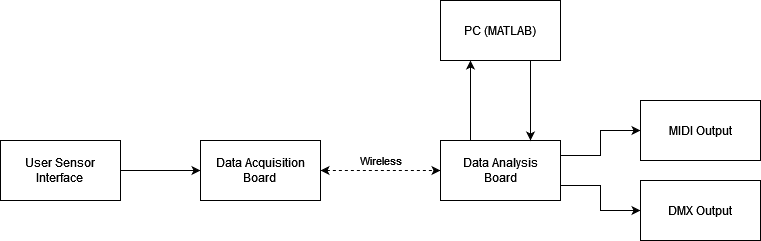
\includegraphics[width=1\columnwidth]{project_plan/figures/System_Block_Diagram}
\end{figure}

\begin{figure}[!ht]
    \caption{Acquisition flow diagram}\label{fig:acquisition}
    \centering
    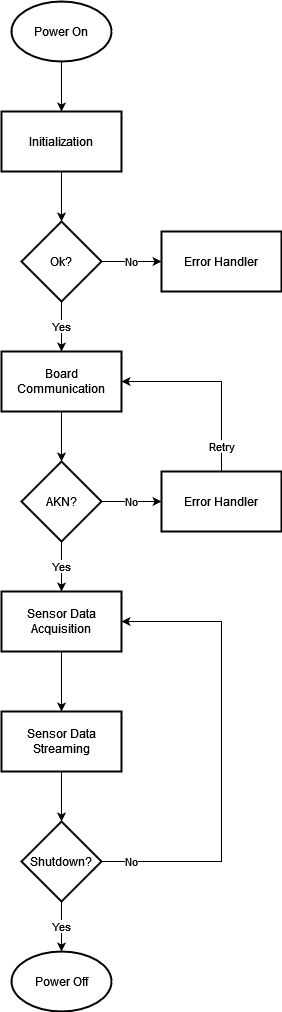
\includegraphics[scale=0.40]{project_plan/figures/Acquisition_Flow_Diagram}
\end{figure}

\begin{figure}[!ht]
    \caption{Analysis flow diagram}\label{fig:analysis}
    \centering
    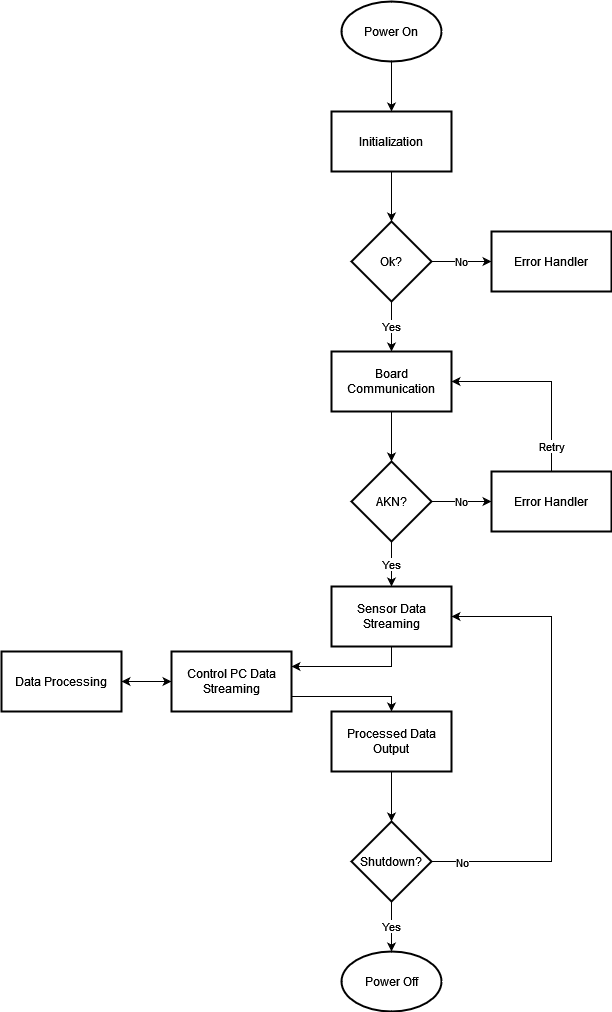
\includegraphics[scale=0.40]{project_plan/figures/Analysis_Flow_Diagram}
\end{figure}

\section{Methodology}
The methodology employed in this project adheres to a structured approach as depicted in \autoref{fig:methodology}.
The initial step involves defining the project objectives and scope in a meticulous and well-defined manner.
Subsequently, a comprehensive market analysis is performed to identify the gap in the market that the project will fulfill.
Based on the analysis, the project requirements are specified, which outline the essential metrics and benchmarks necessary for the project to succeed.
\\
Once the requirements have been established, various options are analyzed and evaluated to determine the most suitable course of action.
The development and prototyping phase follows, where the system is continuously tested to ascertain its conformity with the established requirements.
If the system fails to meet the requirements, the process repeats,
and the analysis, development, and prototyping are redone until the desired outcome is achieved.
Upon successful testing and meeting the requirements, the project moves into the closing phase,
where the project documentation is compiled and handed over to the client.
This approach ensures that the project is executed in a systematic and organized manner,
leading to the delivery of a high-quality product.

\begin{figure}[!ht]
    \caption{Methodology}\label{fig:methodology}
    \centering
    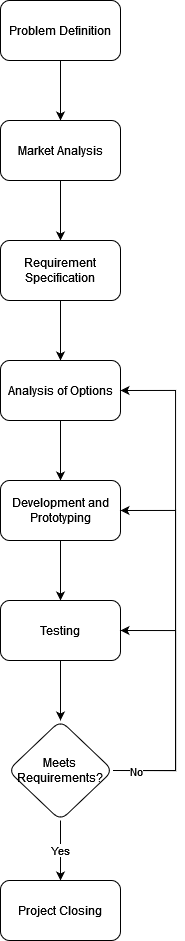
\includegraphics[scale=0.40]{project_plan/figures/Methodology}
\end{figure}

\section{Data Analysis}
The data analysis methodology that will be employed in this project involves a series of steps
to ensure that the collected data is within its usable frequency and at a reasonable magnitude.
First, the sensors that will be used for data collection will be carefully selected and rigorously tested
using specialized equipment such as an oscilloscope.
The data collected from the sensors will then be analyzed to determine the active frequency range and magnitude.
This analysis will inform the design of appropriate filters and amplifiers to be used in the acquisition board.
\\
Once the filters and amplifiers have been designed, the sensors will again be tested to determine if they correctly interface with the acquisition board.
The largest measured value of the sensor will be used to calibrate the acquisition board,
ensuring that the data collected is at the highest resolution possible without loss of information due to clipping.
This process of analysis, design, and testing will be repeated as necessary
to ensure that the sensor data collected is of the highest quality and meets the project requirements.

\section{Work Plan}
A detailed work plan can be found in \autoref{fig:gantt}.
The work plan has been designed to try and maximise the number of concurrent tasks that can be undertaken.
A high level view of the work plan can be found in \autoref{fig:gantt_high_lvl}.

\begin{figure*}[!ht]
    \caption{High level breakdown of gantt chart}\label{fig:gantt_high_lvl}
    \centering
    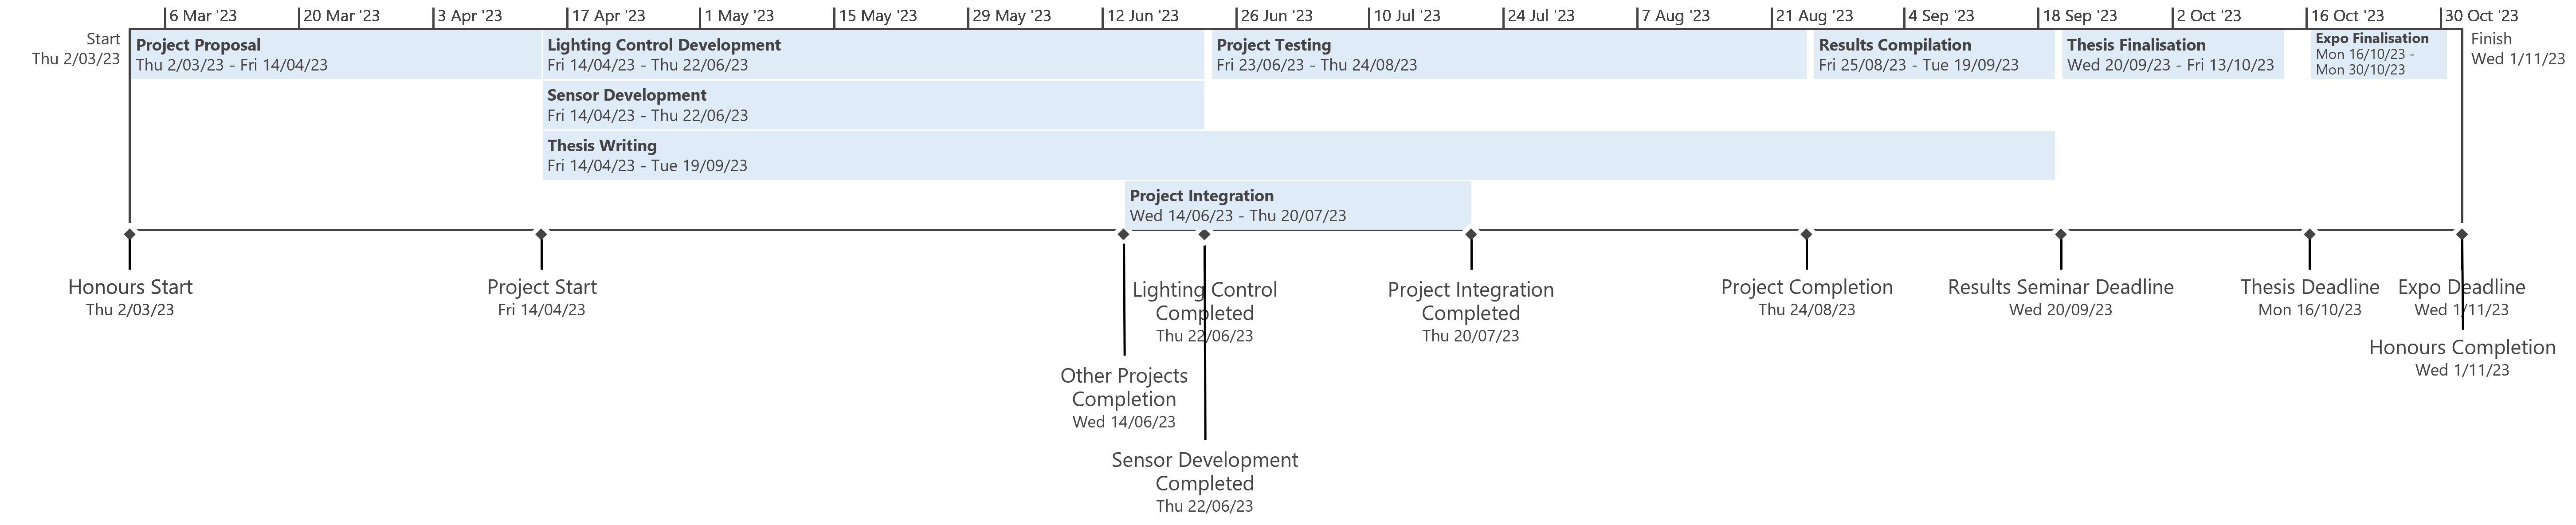
\includegraphics[width=2\columnwidth]{project_plan/figures/Gantt_Chart_High_Level}
\end{figure*}

\begin{figure*}[!ht]
    \caption{Gantt Chart}\label{fig:gantt}
    \centering
    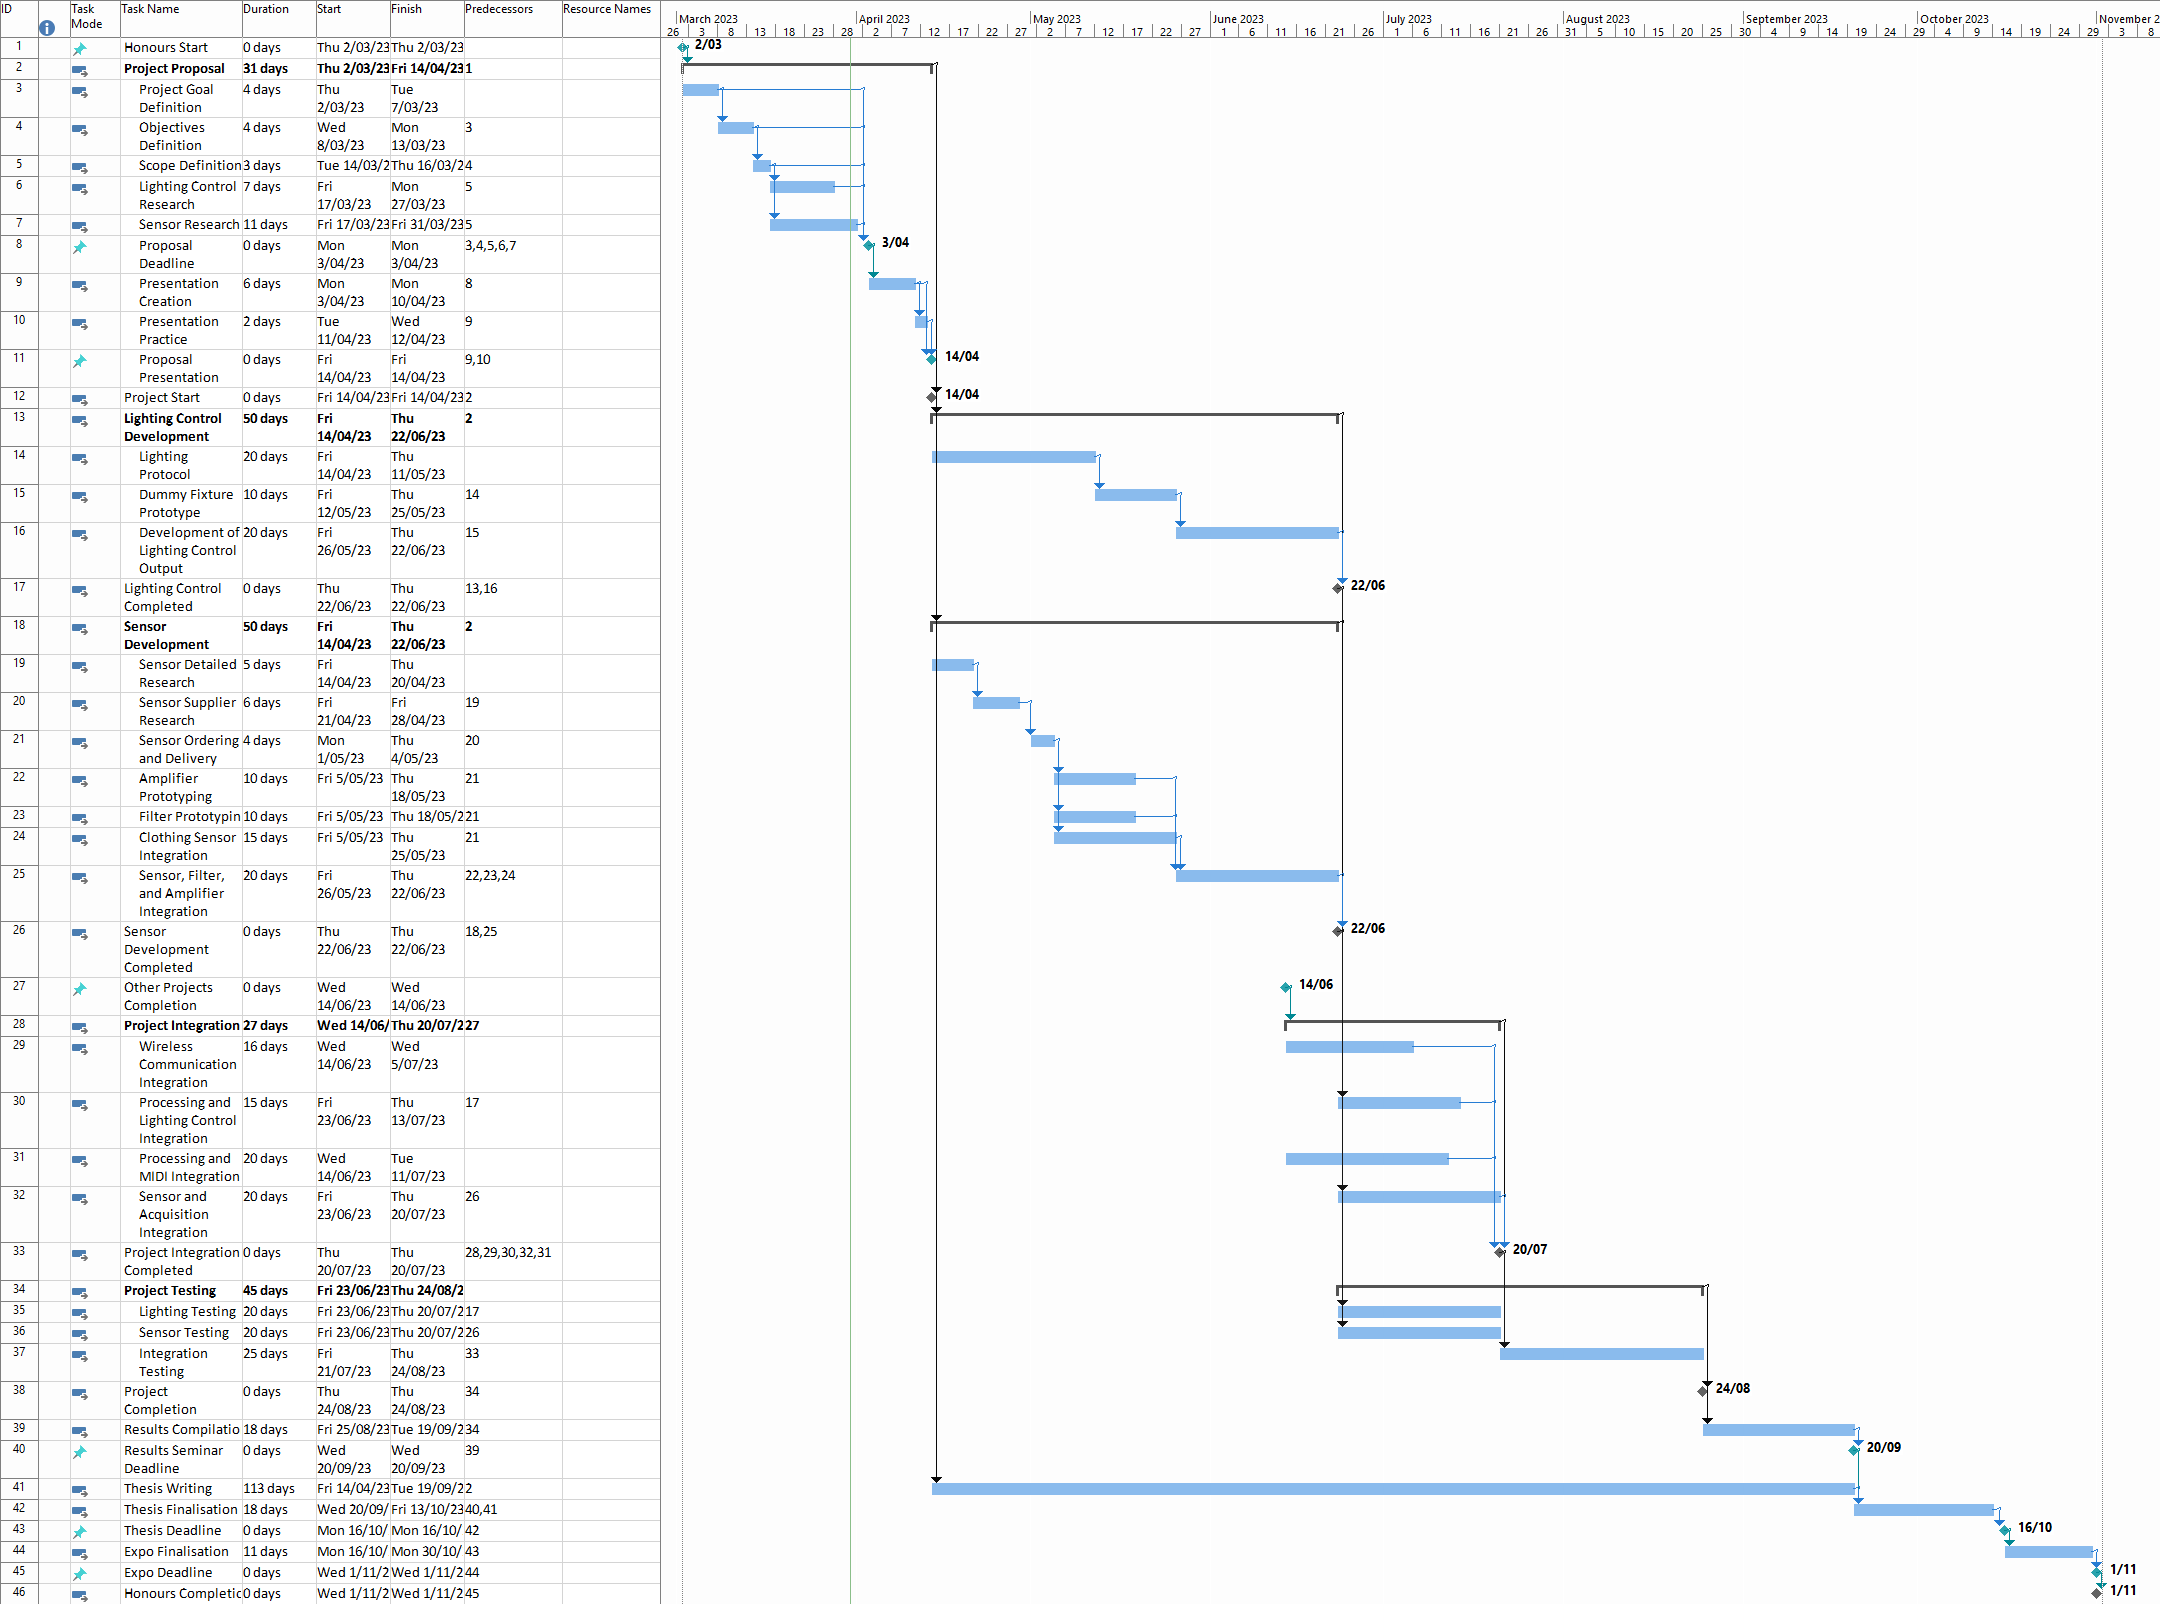
\includegraphics[width=2\columnwidth]{project_plan/figures/Gantt_Chart}
\end{figure*}

\section{Budget}
The total budget of the project cannot exceed the \$600 constraint.
There are a variety of mechanical biosensors that have already been provided for no cost and thus do not need to be purchased.
Of the sensors that will be bought, they will primarily consist of electrode based bio-sensing.
The quoted budget for these sensors are:

\begin{itemize}
    \item \$8.95 for 10 electrodes,
    \item \$10.95 for 10 electrode cables,
    \item \$30 for fingerprint sensor
    \item \$100 for PCB interfaces
\end{itemize}

For a total of \$149.9.
It is important to note that this is an estimated budget,
there are some potential additional costs since the electrodes only have limited uses.
To allow for this, the budget has been set to \$250.

\section{Risk Management}
There are three risks to the success of this project.

The first risk is the lack of DMX equipment to test project functionality with.
This risk can be mitigated by using simulated hardware.
Since the DMX protocol is very well defined,
dummy DMX fixtures can be made using cheap, off-the-shelf microcontrollers.

Secondly, the other honours projects that are underway and completing at the end of this semester.
As the scope of these projects were set before the beginning of this project,
there is a chance that they could encroach on the scope of the project.
To mitigate this risk, the project has been given stretch goals.
This allows the project scope to still be well defined,
while not limiting the scope of the other projects.

The final risk is that the supply chain for electronic components can cause shortages and delays.
This risk has been mitigated by allowing the project to operate using older hardware,
requiring no new stock to be purchased in the case of a supply chain shortage.
In that case, all new suggestions from this project will be considered for future iterations,
and further development will be made modular enough to allow the changes to be implemented.

\section{Conclusion}
Based on the research and analysis conducted,
we propose the development of a system for providing music and lighting control using biological signals.
This system will improve accessibility for musical performance,
while also providing new exciting possibilities to existing performers through biosensor based lighting control.


\chapter{Methodology}
** Assuming at this point what already exists has been clearly researched and shown and the gap in research is clear**

MIGHT BE GOOD TO SKIM THOROUGH PROJECT PLAN AND COMBINE THAT INTO SINGLE HEADING RATHER THAN TRYING TO DO BOTH


\chapter{Results}
** Assuming at this point that the system has been described and the previous contributions are clear, as well as what has been planned to be implemented**

- Lighting Output

- Off-body PC

- On-body Device
    -- ESP32
    -- PIC32
    -- ADS129

- System Integration
The systems works with Xms latency.
The system is able to transmit with 0 bit error rate over 10000 bits.


\chapter{Discussion}
** Assuming at this point what has been achieved has been clearly stated**

Comparing what has been achieved to what has been planned x has happened but y has not.


\chapter{Conclusion}
\chapter{Conclusion}
This project was a continuation of the Music from Biosignals project.
It focussed on developing the hardware for biosignal acquisition, and a controller for controlling lighting fixtures.
The project was successful in creating the lighting controller, as well as programming the hardware.
However, due to previous board design issues, the devices were not able to be powered together.
Therefore, while the device to device connections on the board were tested and working,
the fully system integration was not able to be completed.

This project succeeded in demonstrating the design flaws of the on-body device, while also providing a number of recommendations for a future redesign.


\chapter{Future Work}
\chapter{Future Work}
What can be done going forward


%----------------------------------------------------------------------------------------
%	BIBLIOGRAPHY
%----------------------------------------------------------------------------------------

\printbibliography

%---------------------------------------------------------------------------------------
%	THESIS CONTENT - APPENDICES
%----------------------------------------------------------------------------------------

%\appendix % Cue to tell LaTeX that the following "chapters" are Appendices

% Include the appendices of the thesis as separate files from the Appendices folder
% Uncomment the lines as you write the Appendices

%\include{Appendices/AppendixA}
%\include{Appendices/AppendixB}
%\include{Appendices/AppendixC}

\end{document}
